\section{Geom\-None  Class Reference}
\label{classGeomNone}\index{GeomNone@{Geom\-None}}
A class with no geometry -- a collision never happens. 


{\tt \#include $<$geom.h$>$}

Inheritance diagram for Geom\-None::\begin{figure}[H]
\begin{center}
\leavevmode
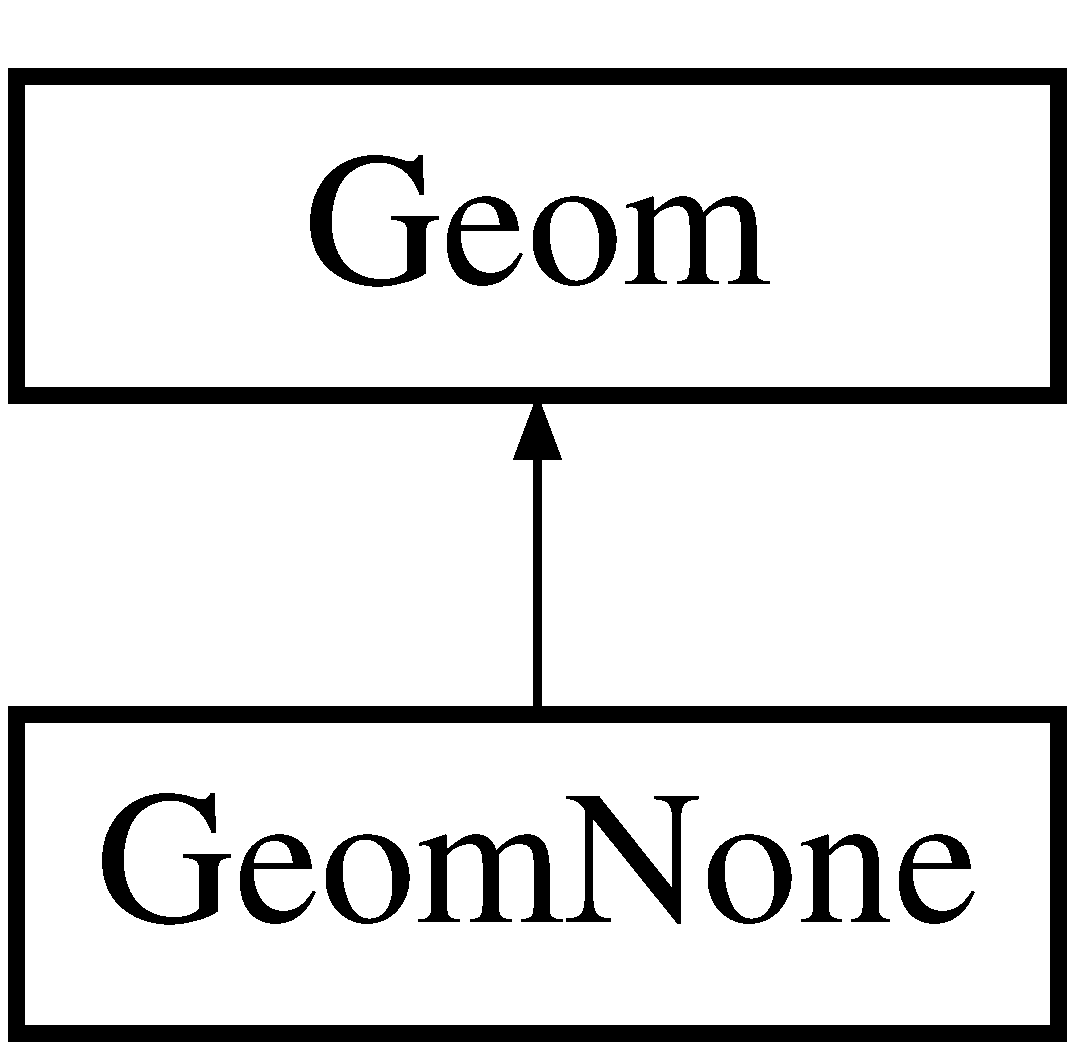
\includegraphics[height=2cm]{classGeomNone}
\end{center}
\end{figure}
\subsection*{Public Methods}
\begin{CompactItemize}
\item 
{\bf Geom\-None} (string path)
\item 
virtual {\bf $\sim$Geom\-None} ()
\item 
virtual bool {\bf Collision\-Free} (const {\bf MSLVector} \&q)
\begin{CompactList}\small\item\em Return true if the robot(s) and obstacles are not in collision.\item\end{CompactList}\item 
virtual double {\bf Distance\-Comp} (const {\bf MSLVector} \&q)
\begin{CompactList}\small\item\em Compute the distance of the closest point on the robot to the obstacle region.\item\end{CompactList}\end{CompactItemize}


\subsection{Detailed Description}
A class with no geometry -- a collision never happens.



\subsection{Constructor \& Destructor Documentation}
\index{GeomNone@{Geom\-None}!GeomNone@{GeomNone}}
\index{GeomNone@{GeomNone}!GeomNone@{Geom\-None}}
\subsubsection{\setlength{\rightskip}{0pt plus 5cm}Geom\-None::Geom\-None (string {\em path} = \char`\"{}\char`\"{})}\label{classGeomNone_a0}


\index{GeomNone@{Geom\-None}!~GeomNone@{$\sim$GeomNone}}
\index{~GeomNone@{$\sim$GeomNone}!GeomNone@{Geom\-None}}
\subsubsection{\setlength{\rightskip}{0pt plus 5cm}Geom\-None::$\sim$Geom\-None ()\hspace{0.3cm}{\tt  [inline, virtual]}}\label{classGeomNone_a1}




\subsection{Member Function Documentation}
\index{GeomNone@{Geom\-None}!CollisionFree@{CollisionFree}}
\index{CollisionFree@{CollisionFree}!GeomNone@{Geom\-None}}
\subsubsection{\setlength{\rightskip}{0pt plus 5cm}bool Geom\-None::Collision\-Free (const {\bf MSLVector} \& {\em q})\hspace{0.3cm}{\tt  [inline, virtual]}}\label{classGeomNone_a2}


Return true if the robot(s) and obstacles are not in collision.



Reimplemented from {\bf Geom} {\rm (p.\,\pageref{classGeom_a2})}.\index{GeomNone@{Geom\-None}!DistanceComp@{DistanceComp}}
\index{DistanceComp@{DistanceComp}!GeomNone@{Geom\-None}}
\subsubsection{\setlength{\rightskip}{0pt plus 5cm}double Geom\-None::Distance\-Comp (const {\bf MSLVector} \& {\em q})\hspace{0.3cm}{\tt  [inline, virtual]}}\label{classGeomNone_a3}


Compute the distance of the closest point on the robot to the obstacle region.



Reimplemented from {\bf Geom} {\rm (p.\,\pageref{classGeom_a3})}.

The documentation for this class was generated from the following files:\begin{CompactItemize}
\item 
{\bf geom.h}\item 
{\bf geom.C}\end{CompactItemize}
